\problemname{Förfalskad snöflinga}
\noindent
Alexander är klimatförnekare, och vill bevisa för Joshua att jorden inte alls blir varmare. 
Alexander menar nämligen att det redan har snöat flera gånger i November, 
vilket snarare tyder på att temperaturen sjunker. Joshua, som mest håller till inomhus, 
har inte märkt av någon snö. 
Därför har Alexander nu sprungit runt och fotat en massa partiklar i luften, 
i hopp om att kunna visa bildbevis för Joshua. 
Nu har han äntligen fått en bild han är ganska nöjd med, 
men han måste göra några ändringar innan han visar bilden. 

Joshua, som älskar fraktaler och onödigt komplicerade saker, har nämligen vissa uppfattningar om hur en snöflinga ska se ut.
En bild består av $N \times N$ pixlar, där $N$ är ett udda tal, och varje pixel antingen är vit eller svart.
Snöflingan utgörs av de vita pixlarna i bilden.
Enligt Joshua föreställer bilden en snöflinga om följande kriterier är uppfyllda:

\begin{itemize}
  \item Mittenpixeln är vit.
  \item Om du roterar bilden medsols 90 grader ser den likadan ut.
  \item Om du speglar bilden längs den vertikala mittlinjen ser den likadan ut.
  \item I bilden finns det inga $2 \times 2$-kvadrater som består helt av vita pixlar. 
  \item Mängden vita pixlar är sammahängande \emph{utan diagonala steg}. 
    Detta innebär att om du börjar med en penna på någon vit pixel, kan 
    du komma åt varje annan vit pixel utan att lyfta pennan och utan
    att rita på svarta pixlar.
    Pennan får gå upp, ned, vänster och höger, \emph{men inte} diagonalt.
  \item Mängden svarta pixlar är sammanhängande \emph{med diagonala steg}.
    Detta innebär att om du börjar med en penna på någon svart pixel, kan 
    du komma åt varje annan svart pixel utan att lyfta pennan och utan
    att rita på vita pixlar.
    Pennan får gå upp, ned, vänster, höger, \emph{och} diagonalt.

\begin{centering}
    \begin{figure}[h]
        \centering
        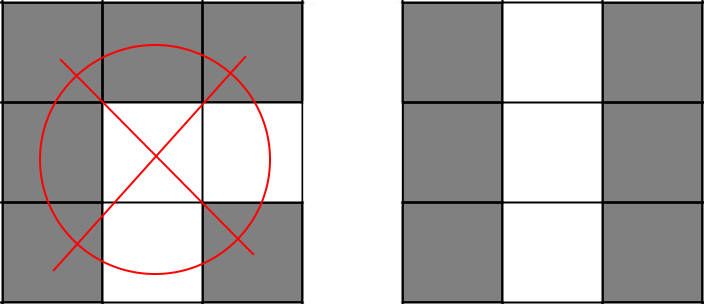
\includegraphics[scale=0.2]{crook_example.png}
        \caption{Två stycken $3\times 3$-bilder. De tre pixlarna till vänster utgör en krok, vilket inte är tillåtet. De tre pixlarna till höger utgör inte en krok.}
        \label{fig:enter-label}
    \end{figure}
\end{centering}
    
  \item Det finns inga krokar i snöflingan. 
  Låt $\text{pixel}_\text{upp}$, $\text{pixel}_\text{höger}$, $\text{pixel}_\text{ner}$, och $\text{pixel}_\text{vänster}$ vara de angränsande 
  pixlarna till en vit pixel. En krok uppstår om precis två av dessa angränsande pixlar också är vita, och de inte är på motsatta sidor av pixeln.
  Alltså, om till exempel $\text{pixel}_\text{upp}$ och $\text{pixel}_\text{höger}$ är vita medan $\text{pixel}_\text{ner}$ 
  och $\text{pixel}_\text{vänster}$ är svarta uppstår en krok, men om $\text{pixel}_\text{upp}$ och $\text{pixel}_\text{ner}$ är vita
  och $\text{pixel}_\text{höger}$ och $\text{pixel}_\text{vänster}$ är svarta uppstår inte en krok.
      
\end{itemize}

\begin{centering}
    \begin{figure}[h]
        \centering
        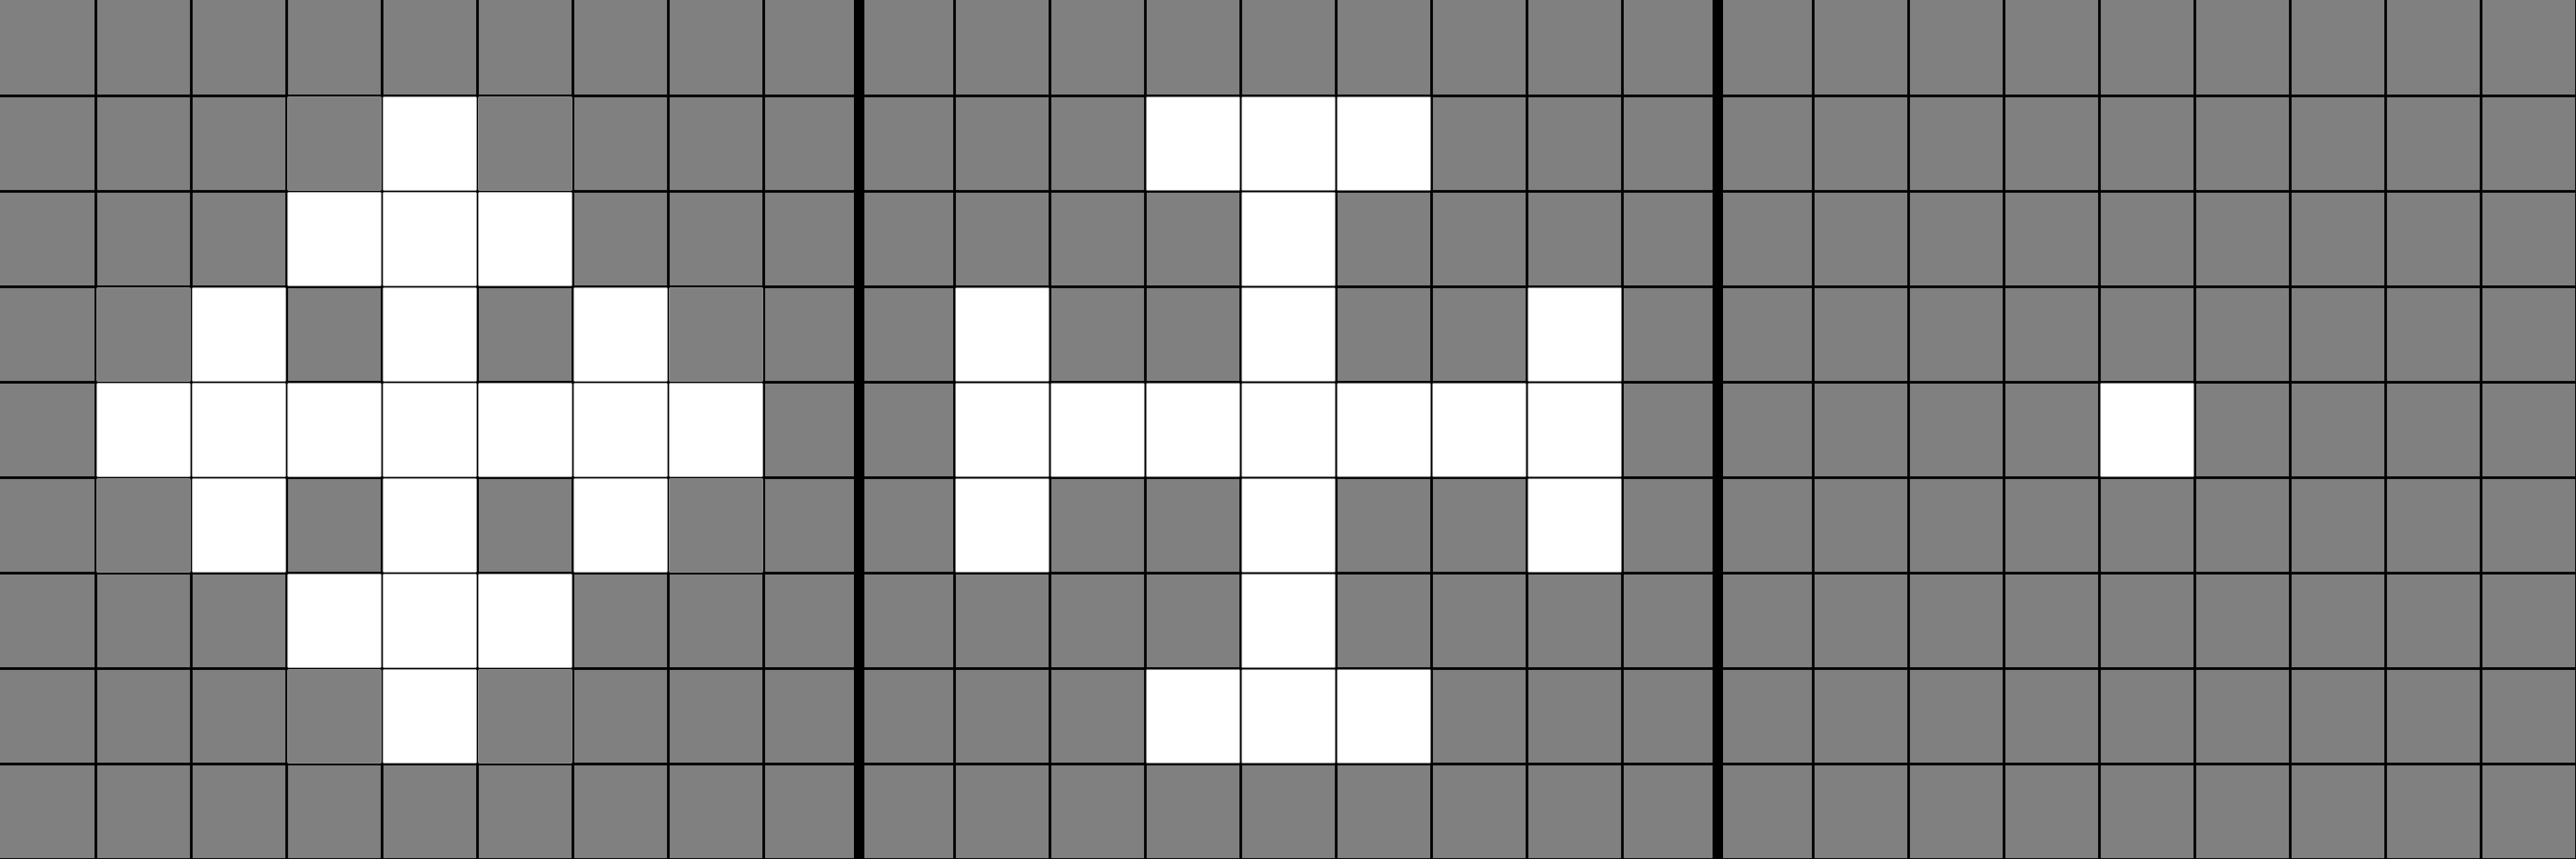
\includegraphics[scale=0.1]{all_valid_examples.png}
        \caption{Tre exempel på $9\times 9$-bilder som visar snöflingor.}
        \label{fig:enter-label}
    \end{figure}
\end{centering}

\begin{centering}
    \begin{figure}[h]
        \centering
        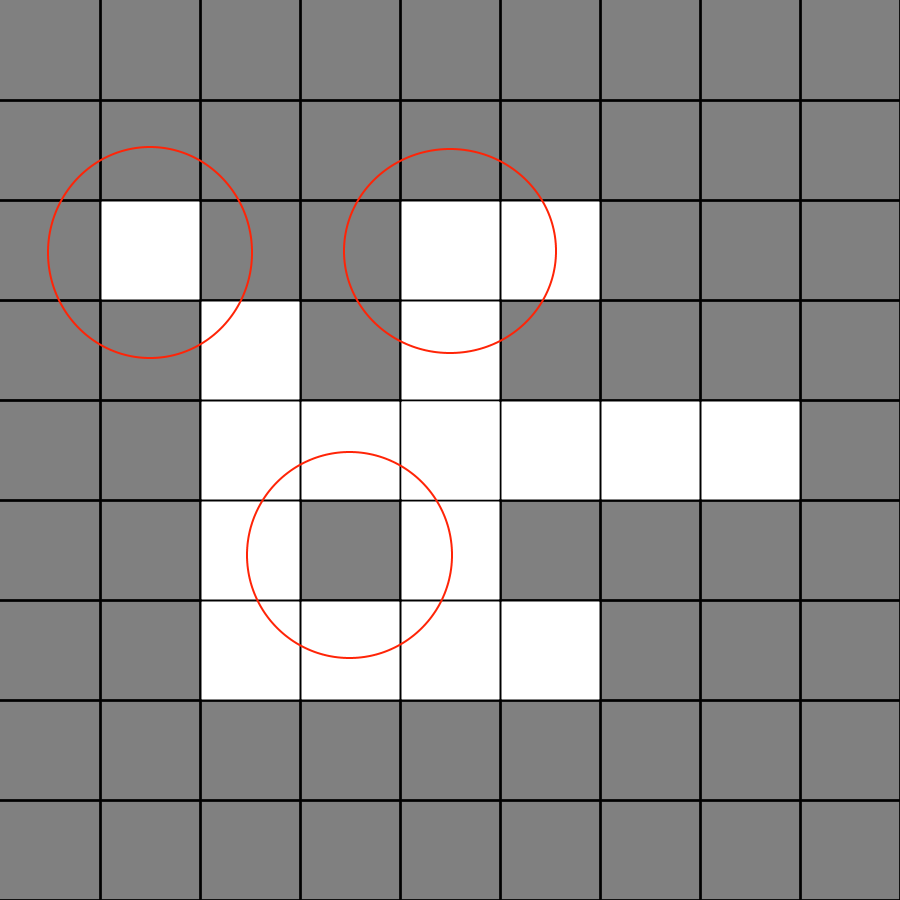
\includegraphics[scale=0.1]{invalid_example.png}
        \caption{En väldigt felaktig snöflinga. Av de tre inringade pixlarna finns en vit pixel ej sammanhängande med resten av de vita, en pixel som utgör en krok, och en svart pixel ej sammanhängande med resten av de svarta. Dessutom uppfyller bilden inte något av de två symmetrikraven.}
        \label{fig:enter-label}
    \end{figure}
\end{centering}

\noindent
Alexander har laddat ner ett bildredigerarprogram där han kan ändra färgen på pixlar, både från svart till vitt och från vitt till svart. 
Eftersom han inte är så duktig på bildredigering räknar Alexander med att det tar honom en minut för varje pixel han behöver ändra.
Alexander är en väldigt upptagen man, och vill därför vara så tidseffektiv som möjligt.
Han vill nu veta hur snabbt han kan vara innan han blir färdig med redigeringen, om han ändrar så få pixlar som möjligt. 

\section*{Indata}
Den första raden i indatan innehåller det udda heltalet $N$ ($7 \le N \le 15$), antalet pixlar på sidan av den kvadratiska bilden.
Därefter följer $N$ rader, där den $i$:te raden innehåller de $N$ talen $p_{i,1}, p_{i,2}, ..., p_{i,N}$.
Om pixeln på position ($i$, $j$) i bilden är vit så är $p_{i,j} = 1$, annars är $p_{i,j} = 0$.
Position (1,1) motsvarar pixeln högst upp i vänstra hörnet.

\section*{Utdata}
Skriv ut ett heltal: Det minsta antalet minuter det tar Alexander att ändra i sin bild för att Joshua
ska gå med på att bilden föreställer en snöflinga.


\section*{Poängsättning}
Din lösning kommer att testas på en mängd testfallsgrupper.
För att få poäng för en grupp så måste du klara alla testfall i gruppen.

\noindent
\begin{tabular}{| l | l | p{12cm} |}
  \hline
  \textbf{Grupp} & \textbf{Poäng} & \textbf{Gränser} \\ \hline
  $1$    & $20$       & $N=7$ \\ \hline
  $2$    & $20$       & $N=11$ \\ \hline
  $3$    & $60$       & $N=15$ \\ \hline
\end{tabular}

